% !TEX program = xelatex
\documentclass[notes=hide]{beamer}
%\documentclass[notes=onlyslideswithnotes,notes=hide]{beamer}
%\documentclass[notes=only]{beamer}
%\documentclass[11pt,letterpaper]{article}
%\usepackage{beamerarticle}

\usepackage{analchem}
\usepackage{lecture}
\usepackage{multicol}
\renewcommand*\printatom[1]{\ensuremath{\mathsf{#1}}}
\usepackage{pgfplots}
\pgfplotsset{compat=1.3}
\usepackage{cancel}

\title{Acid-Base Equilibria}
\subtitle{Chapters 9-11}
\institute{CHEM321 --- Analytical Chemistry I \\ Bloomsburg University}
\author{D.A. McCurry}
\date{Fall 2020}

\begin{document}

\maketitle
\mode<article>{\thispagestyle{fancy}}

\frame{\section{Systematic Treatment of Acid-Base Equilibria}
	\begin{learningobjectives}
	\item Apply the systematic treatment of equilibria specifically to acid-base reactions.
	\item Understand that approximations are less accurate as concentrations become more dilute.
	\end{learningobjectives}
}

\begin{frame}{\ch{HNO3} --- One of our Strong Acids}
	\begin{columns}
		\column{0.5\linewidth}
		\begin{center}
			\includegraphics[scale=0.3]{HNO3Raman.jpeg}
			*undissociated \ch{HNO3}
		\end{center}
		\column{0.5\linewidth}
		\begin{center}
			\includegraphics[scale=0.5]{HNO3Dissociation.jpeg}
			\includegraphics[scale=0.5]{HNO3TempKa.jpeg}
		\end{center}
	\end{columns}
\end{frame}

\begin{frame}{The Hazard of $\text{pH} = -\log[\ch{H3O+}]$}
	As we've seen, calculating pH of strong acids and bases is very easy
	because they dissociate 100\%:
	\begin{reaction*}
		!( "\SI{0.0100}{\Molar}" )( HNO3 ) -> !( "\SI{0.0100}{\Molar}" )( H3O+ ) + !( "\SI{0.0100}{\Molar}" )( NO3- )
	\end{reaction*}
	\begin{equation*}
		\therefore \pH = -\log(0.0100) = 2.000
	\end{equation*}

	\pause

	\begin{reaction*}
		!( "\SI{1.00e-8}{\Molar}" )( HNO3 ) -> !( "\SI{1.00e-8}{\Molar}" )( H3O+ ) + !( "\SI{1.00e-8}{\Molar}" )( NO3- )
	\end{reaction*}
	\begin{equation*}
		\therefore \pH = -\log(\num{1.00e-8}) = 8.000
	\end{equation*}

	\pause

	What happened? Why did this stop working?
\end{frame}

\vspace{\stretch{-1}}

\begin{frame}{A Systematic Approach to pH}
	\note{
	\begin{enumerate}
		\item Pertinent Reactions
			\begin{align*}
				\ch{!( "\SI{1.00e-8}{\Molar}" )( HNO3 ) &-> !( "\SI{1.00e-8}{\Molar}" )( H3O+ ) + !( "\SI{1.00e-8}{\Molar}" )( NO3- )} \\
				\ch{2 H2O &<=> H3O+ + OH-}
			\end{align*}
	\end{enumerate}
	\begin{multicols}{2}
		\begin{enumerate}
			\setcounter{enumi}{1}
			\item Charge Balance
				\begin{align*}
					[\ch{H3O+}] = [\ch{OH-}] + [\ch{NO3-}]
				\end{align*}
			\item Mass Balance
				\begin{align*}
					[\ch{NO3-}] = \SI{1.00e-8}{\Molar}
				\end{align*}
			\item Write K's
				\begin{align*}
					K_w = [\ch{H3O+}][\ch{OH-}]
				\end{align*}
			\item Count: 3 unknowns and 3 equations!
			\item Solve
		\end{enumerate}
	\end{multicols}
	}

\end{frame}

\note{\footnotesize
	Substitute the MB into the CB:
	\begin{align*}
		[\ch{H3O+}] &= [\ch{OH-}] + \SI{1.00e-8}{\Molar} \\[1em]
		\shortintertext{Rearrange for easier solving:}
		[\ch{OH-}] &= [\ch{H3O+}] - \SI{1.00e-8}{\Molar} \\[1em]
		\shortintertext{Plug into $K_w$ expression:}
		\num{1.0e-14} &= [\ch{H3O+}]([\ch{H3O+}] - \num{1.00e-8}) \\
		0 &= [\ch{H3O+}]^2 - \num{1.00e-8}[\ch{H3O+}] - \num{1.0e-14} \\
		[\ch{H3O+}] &= \SI{1.05e-7}{\Molar} \text{ and }
		\fbox{\text{pH}=6.98}
	\end{align*}

	There are 2 sources of \ch{H3O+} in any aqueous acid solution -- the acid
	and the water.
}

\clearpage

\begin{frame}[shrink]{Spreadsheet software aids in pH determination}
	\begin{tabular} {S[table-format=1.1e-2] *{2}{S[table-format=2.2]} || S[table-format=1.1e-2]
		*{2}{S[table-format=2.2]}}
		\toprule
		{[Strong Acid]} & {$\approx$ pH} & {$=$ pH} & {[Strong Base]} & {$\approx$ pH} & {$=$ pH} \\ \midrule
		1.0e-1 & 1.00 & 1.00   & 1.0e-1 & 13.00 & 13.00 \\
		1.0e-2 & 2.00 & 2.00   & 1.0e-2 & 12.00 & 12.00 \\
		1.0e-3 & 3.00 & 3.00   & 1.0e-3 & 11.00 & 11.00 \\
		1.0e-4 & 4.00 & 4.00   & 1.0e-4 & 10.00 & 10.00 \\
		1.0e-5 & 5.00 & 5.00   & 1.0e-5 & 9.00 & 9.00   \\
		1.0e-6 & 6.00 & 6.00   & 1.0e-6 & 8.00 & 8.00   \\
		1.0e-7 & 7.00 & 6.79   & 1.0e-7 & 7.00 & 7.21   \\
		1.0e-8 & 8.00 & 6.98   & 1.0e-8 & 6.00 & 7.02   \\
		1.0e-9 & 9.00 & 7.00   & 1.0e-9 & 5.00 & 7.00   \\
		1.0e-10 & 10.00 & 7.00 & 1.0e-10 & 4.00 & 7.00  \\
		1.0e-11 & 11.00 & 7.00 & 1.0e-11 & 3.00 & 7.00  \\
		1.0e-12 & 12.00 & 7.00 & 1.0e-12 & 2.00 & 7.00  \\
		\bottomrule
	\end{tabular}
\end{frame}


\begin{frame}{Even better\ldots we can plot it!}
	\centering
	\includegraphics[width=\textwidth]{strongacid-base.eps}
\end{frame}


\begin{frame}[shrink]{How much \ch{H3O+} comes from water?}
	\only<+>{%
	\begin{tabular} {S[table-format=1.1e-2]
		S[table-format=1.1e-2] S[table-format=3.3]
		S[table-format=1.1e-2] S[table-format=3.10]}
		\toprule
		& \multicolumn{2}{c}{From acid} & \multicolumn{2}{c}{From
		water} \\
		{[Strong Acid]} & [\ch{H3O+}] & \% & [\ch{H3O+}] & \% \\ \midrule
		1.0e-1 & 1.0e-1 & 100 & 1.0e-13 & 0.0000000001 \\
		1.0e-2 & 1.0e-2 & 100 & 1.0e-12 & 0.00000001 \\
		1.0e-3 & 1.0e-3 & 100 & 1.0e-11 & 0.000001 \\
		1.0e-4 & 1.0e-4 & 100 & 1.0e-10 & 0.0001 \\
		1.0e-5 & 1.0e-5 & 100 & 1.0e-9 & 0.01 \\
		1.0e-6 & 1.0e-6 & 99 & 9.9e-9 & 1 \\
		1.0e-7 & 1.0e-7 & 62 & 6.2e-8 & 38 \\
		1.0e-8 & 1.0e-8 & 10 & 9.5e-8 & 90 \\
		1.0e-9 & 1.0e-9 & 1 & 1.0e-7 & 99 \\
		1.0e-10 & 1.0e-10 & 0.1 & 1.0e-7 & 100 \\
		1.0e-11 & 1.0e-11 & 0.01 & 1.0e-7 & 100 \\
		1.0e-12 & 1.0e-12 & 0.001 & 1.0e-7 & 100 \\
		\bottomrule
	\end{tabular}
}

\only<+>{%
	\noindent
	If we have \SI{1.0e-2}{\Molar} \ch{HNO3}, the \ch{OH-} concentration
	follows,

	\begin{align*}
		[\ch{OH-}] &= \dfrac{\num{1.0e-14}}{[\ch{H3O+}]} \\
		&= \dfrac{\num{1.0e-14}}{\num{1.0e-2}} = \SI{1.0e-12}{\Molar}
	\end{align*}

	The \alert{only} source of \ch{OH-} is the dissociation of water, so
	water must \emph{also} contribute \SI{1.0e-12}{\Molar} \ch{H3O+}!
}
\end{frame}

\frame{\section{Weak Acids and Bases}
	\begin{learningobjectives}
	\item Apply the systematic treatment of equilibria to weak acids and bases.
	\item Know when certain approximations may be used to simplify calculations.
	\item Understand the fractional dissociation/association of weak acids and bases.
	\end{learningobjectives}
	}

\begin{frame}{Weak Acids and Bases}
	\begin{block}{Weak Acid Equilibrum}
		\begin{align*}
			\ch{HA + H2O <=>[ $K_a$ ] H3O+ + A-} \qquad K_a =
			\dfrac{[\ch{H+}][\ch{A-}]}{[\ch{HA}]}
		\end{align*}
	\end{block}

	\begin{block}{Weak Base Equilibrum}
		\begin{align*}
			\ch{B + H2O <=>[ $K_b$ ] BH+ + OH-} \qquad K_b =
			\dfrac{[\ch{BH+}][\ch{OH-}]}{[\ch{B}]}
		\end{align*}
	\end{block}

	Conjugate Acid-Base Pairs: $K_a \times K_b = K_w$
\end{frame}

\vspace{\stretch{-1}}

\begin{frame}[t]{A Typical Weak Acid Problem}
	Find the pH of a solution of the weak acid, HA, given the formal
	concentration of HA and the value of \Ka.

	\mode<article>{\vfill}

	\note{
		\begin{multicols}{2}
		\begin{enumerate}
			\item Pertinent equations:
				{\footnotesize
				\begin{align*}
					\ch{HA + H2O &<=>[ $K_a$ ] H3O+ + A-} \\
					\ch{2 H2O &<=>[ $K_w$ ] H3O+ + OH-}
				\end{align*}}
			\item Charge Balance:
				{\footnotesize
				\begin{align*}
					[\ch{H3O+}] = [\ch{OH-}] + [\ch{A-}]
				\end{align*}}
			\item Mass Balance:
				{\footnotesize
				\begin{align*}
					\si{\formal} = [\ch{A-}] + [\ch{HA}]
				\end{align*}}
			\item Equilibria:
				{\footnotesize
				\begin{align*}
					\Ka &= \frac{[\Oxo][\ch{A-}]}{[\ch{HA}]} \\
					\Kw &= [\Oxo][\Hyd]
				\end{align*}}
			\item Count: 4 unknowns and 4 equations, then
			\item Solve!
		\end{enumerate}
		\end{multicols}
		\begin{align*}
			0 = [\Oxo]^3 + [\Oxo]^2\Ka -
			[\Oxo](\si{\formal}\Ka + \Kw) - \Kw\Ka
		\end{align*}
	}
\end{frame}

\begin{frame}[t]{``Wait!''}
	The Good Chemist comes galloping down from the mountain on her white
	stallion to rescue us. ``There is no reason to solve a cubic equation.
	We can make an excellent, simplifying approximation.''

	\begin{itemize}
		\item The amount of \ch{H3O+} from the acid is much larger than
			that from water at \alert{normal lab concentrations}.
			\begin{align*}
				[\ch{A-}] >> [\ch{OH-}] \qquad\therefore [\ch{H3O+}]
				\approx [\ch{A-}]
			\end{align*}
		\item Let $x = [\Oxo] = [\ch{A-}]$
%			If $x = [\ch{H3O+}]$, then
%			\begin{align*}
%				[\ch{H3O+}] &= [\ch{A-}] = x \\
%				\textsc{F} &= [\ch{A-}] + [\ch{HA}] \qquad\therefore
%				[\ch{HA}] = \textsc{F} - x \\
%				K_a &= \dfrac{[\ch{H+}][\ch{A-}]}{[\ch{HA}]} =
%				\dfrac{x^2}{\textsc{F}-x}
%			\end{align*}
	\end{itemize}

	\clearpage

	\mode<article>{\vspace*{\stretch{0.5}}}

	\note{\begin{multicols}{2}
		\begin{enumerate}
			\item Pertinent equations:
				{\footnotesize
				\begin{align*}
					\ch{HA + H2O &<=>[ $K_a$ ] H3O+ + A-} \\
					\ch{2 H2O &<=>[ $K_w$ ] H3O+ + OH-}
				\end{align*}}
			\item Charge Balance:
				{\footnotesize
				\begin{align*}
					x &= [\Hyd] + x \\
					\therefore [\Hyd] &= 0
				\end{align*}}
			\item Mass Balance:
				{\footnotesize
				\begin{align*}
					\si{\formal} &= x + [\ch{HA}] \\
					\therefore [\ch{HA}] &= \si{\formal} - x
				\end{align*}}
			\item Equilibria:
				{\footnotesize
				\begin{align*}
					\Ka &= \frac{x^2}{[\ch{HA}]} = \boxed{\frac{x^2}{\si{\formal} - x}} \\
					\Kw &= x [\ch{OH-}] \approx 0
				\end{align*}}
			\item Count: 4 unknowns and 4 equations, then
			\item Solve!
		\end{enumerate}
		\end{multicols}
	}
\end{frame}

\begin{frame}[t]{Weak Acid Example}
	What is the \pH{} of a \SI{0.0500}{\Molar} \para-hydroxybenzoic acid ($\pKa =
	4.54$) solution?

	\note{\begin{align*}
		\Ka &= \num{2.9e-5} = \dfrac{x^2}{\si{\formal} - x} =
		\dfrac{x^2}{\num{0.0500} - x} \\
		0 &= x^2 + \num{2.9e-5}x - \num{1.45e-6} \\
		\intertext{After some quadratic magic:}
		x &= [\ch{H3O+}] = [\ch{A-}] = \SI{1.2e-3}{\Molar} \\
		\pH &= \boxed{2.92} \\
		\therefore \pOH &= 11.08 \\
		[\ch{OH-}] &= \SI{8.4e-12}{\Molar}
	\end{align*}
	\SI{8.4e-12}{\Molar} \ch{H3O+} comes from \ch{H2O}, so it is a valid
assumption that 100\% of \ch{H3O+} comes from HA and none from \ch{H2O}!}
\end{frame}

\clearpage

\begin{frame}{Fraction of Dissociation}
	\begin{columns}
		\column{0.55\textwidth}
		Amount dissociated relative to the mass balance or total amount.
		\begin{align*}
			\alpha = \frac{[\ch{A-}]}{[\ch{HA}] + [\ch{A-}]} =
			\frac{x}{\si{\formal}}
		\end{align*}
		For the last example,
		\begin{align*}
			\alpha =
			\frac{\SI{1.2e-3}{\Molar}}{\SI{0.0500}{\Molar}} =
			\fbox{0.024 = 2.4\%}
		\end{align*}
		\begin{center}
			\includegraphics[scale=0.5]{hydroxybenzoic-acid.jpeg}
		\end{center}
		\column{0.45\textwidth}
		\begin{center}
			\includegraphics[scale=0.33]{frac-dissociation.jpeg}
		\end{center}
	\end{columns}
\end{frame}

\begin{frame}{Weak Base Equilibria}
	We can make the same assumption as with the weak acids, i.e., that
	nearly all the \ch{OH-} comes from the weak base and very little from
	the water.

	\begin{align*}
		\ch{B + H2O &<=> HB+ + OH-} &\qquad \Kb &=
		\frac{[\ch{HB+}][\ch{OH-}]}{[\ch{B}]} \\
		[\ch{B}] &= \si{\formal} - [\ch{HB+}] = \si{\formal} - x &\qquad
		\therefore \Kb &= \frac{x^2}{\si{\formal}-x}
	\end{align*}
\end{frame}

\begin{frame}[t]{Weak Base Example}
	What is the pH of a \SI{0.00372}{\Molar} cocaine solution?

	\begin{center}
		\includegraphics[scale=0.25]{base-association.jpeg}
	\end{center}

	\mode<article>{\vfill}

	\note{
		\begin{reaction*}
%			B + \water <=> HB+ + \Hyd
			!($0.00372-x$)( B ) + \water <=> !($x$)( HB+ ) + !($x$)(\Hyd)
		\end{reaction*}
		
		\begin{align*}
			\Kb &= \frac{x^2}{\si{\formal} - x} \\
			\num{2.6e-6} &= \frac{x^2}{0.00372-x} \\
			\intertext{via quadratic,}
			x &= \SI{9.71e-5}{\Molar}~\Hyd \\
			\therefore [\Oxo] &= \SI{1.03e-10}{\Molar} \text{~and~} \pH{} = 9.99
		\end{align*}
	}
\end{frame}

\begin{frame}{Fraction of Association}
	\begin{align*}
		\alpha = \frac{[\ch{HB+}]}{[\ch{B}] + [\ch{HB+}]} =
		\dfrac{x}{\si{\formal}}
	\end{align*}

	For the last example,

	\begin{align*}
		\alpha =
		\frac{\SI{9.71e-5}{\Molar}}{\SI{3.73e-3}{\Molar}} =
		\fbox{0.0260 = 2.60\%}
	\end{align*}

	\begin{block}{Fraction of Association/Dissociation}
		\begin{align*}
			\frac{x}{\si{\formal}} = \frac{\text{amount
			associated/dissociated}}{\text{total amount of species}}
		\end{align*}
	\end{block}
\end{frame}

\vspace{\stretch{-1}}

\clearpage

\frame{\section{Buffers}
	\begin{learningobjectives}
	\item Describe the utility of buffers in chemical analysis.
	\item Calculate buffer capacity and useful \pH{} range for a buffer.
	\item Prepare a buffer of desired \pH{}.
	\end{learningobjectives}
	}

\vspace{\stretch{-1}}

\begin{frame}[t]{Buffers}
	\begin{itemize}[<+->]
		\item What is a buffer?
		\item What is it used for?
	\end{itemize}

	\note<.>{%
		\begin{align*}
			\Ka &= \frac{[\Oxo][\ch{A-}]}{[\ch{HA}]} \\
			\log\Ka &= \log[\Oxo] + \log\frac{[\ch{A-}]}{[\ch{HA}]} \\
			-\log[\Oxo] &= -\log\Ka + \log\frac{[\ch{A-}]}{[\ch{HA}]} \\
			\pH &= \pKa + \log\frac{[\ch{A-}]}{[\ch{HA}]} \\
			\text{or, for a base:} \qquad
			\pH &= \pKa + \log\frac{[\ch{B}]}{[\ch{HB+}]} \\
		\end{align*}
	}

	\vspace{\stretch{2}}

	\begin{block}<+->{The Henderson-Hasselbalch Equation}
		\begin{columns}
			\column{0.45\linewidth}
			\begin{align*}
				\pH &= \pKa + \log\frac{[\ch{A-}]}{[\ch{HA}]}
			\end{align*}
			\begin{itemize}
				\item Easy \pH{} calculation.
				\item Indicates buffer capacity.
				\item Helps identify \emph{principal
					species} in a solution.
			\end{itemize}
			\column{0.45\linewidth}
			\begin{tabular} {r@{/}l l}
				\multicolumn{2}{c}{[\ch{A-}]/[\ch{HA}]} &
				\multicolumn{1}{c}{\pH} \\ \midrule
				100 & 1   & $\pKa + 2$ \\
				10  & 1   & $\pKa + 1$ \\
				1   & 1   & $\pKa$ \\
				1   & 10  & $\pKa - 1$ \\
				1   & 100 & $\pKa - 2$
			\end{tabular}
		\end{columns}
	\end{block}
\end{frame}

\mode<presentation>{
\begin{frame}{Alkaline Water}
	\centering
	\includegraphics[width=0.6\textwidth]{alkaline-water.pdf}
	\footnote{https://www.mayoclinic.org}
\end{frame}}

\vspace{\stretch{-1}}

\clearpage

\begin{frame}[t]{Henderson-Hasselbalch Example}
	We have \SI{200.}{\milli\liter} of a solution containing
	\SI{0.250}{\Molar} citric acid and \SI{0.200}{\Molar} sodium citrate. To
	this, \SI{10.0}{\milli\liter} of \SI{0.750}{\Molar}~\ch{NaOH} is added.
	What is the change in \pH?

	\note{
		\begin{enumerate}
			\item Initial \pH:
				\begin{align*}
					\pH &= \pKa + \log\frac{[\ch{A-}]}{[\ch{HA}]} \\
					&= 3.13 + \log\frac{0.200}{0.250} = 3.03
				\end{align*}
			\item Adding base, so reacting? \textbf{Citric Acid}
			\item ICE:
		\begin{tabular} {*{7}{r} l}
			\ch{HA} & + & \ch{OH-} & \ch{<=>} & \ch{A-} & + &
			\ch{H2O} \\
			50.0 & & 7.50 & & 40.0 & & & \si{\milli\mole} each \\
			-7.50 & & -7.50 & & +7.50 & & & \si{\milli\mole} each 
		\end{tabular}
	\end{enumerate}

		\begin{align*}
			\text{pH} = 3.13 + \log\dfrac{47.5}{42.5} = 3.18 \qquad
			\fbox{\textrm{d}\text{pH} = +0.15}
		\end{align*}
		}
\end{frame}

\begin{frame}{Preparing a buffer}
	\only<1-5>{%
	You can calculate the appropriate mass of each component and dissolve in
	appropriate volume to make the appropriate buffer.
	\begin{itemize}[<+(1)->]
		\item Activity coefficients
			\begin{block}<1->{The Real Henderson-Hasselbalch Equation}
				Diluting buffers can significantly change \pH!
				\begin{equation*}
					\pH = \pKa +
					\log\frac{[\ch{A-}]\gamma_{\ch{A-}}}{[\ch{HA}]}
				\end{equation*}
			\end{block}
		\item \pKa is often listed at
			\SI{25}{\celsius} which \emph{may not
			be true} in lab
		\item Approximations (``Good chemist'') might
			not be accurate enough
		\item Other ion contributions
	\end{itemize}
}

\only<6->{%
	Instead, weigh a quantity of acid (or base) for desired concentration
	and add water to \emph{near desired} volume. Add a \emph{strong} base
	(or acid) until the desired \pH is reached, then dilute to desired
	volume.
	\begin{itemize}
		\item<7-> Strong species will alter
			[\ch{A-}]/[\ch{HA}] ratio by
			\emph{consuming} (neutralizing)
			species.
		\item<8-> Why do we have to add water first?
	\end{itemize}
}
\end{frame}

\vspace{\stretch{-1}}
\clearpage

\begin{frame}{Buffer Capacity}
	\begin{columns}
		\column{0.5\linewidth}
		A measure of how well a solution resists changes in \pH{} when a
		strong acid or base is added.
		\begin{align*}
			\beta = \frac{\textrm{d}C_b}{\textrm{d}\pH} =
			-\frac{\textrm{d}C_a}{\textrm{d}\pH} 
		\end{align*}
		where $C_b$ and $C_a$ are the moles of the strong acid and base
		needed to change 1 liter of buffer by 1 pH unit.
		\column{0.4\linewidth}
		\begin{center}
			\includegraphics[scale=0.33]{buffercap.jpeg}
			
			\footnotesize
			\SI{0.100}{\formal} \ch{HA} with $\pKa = 5$
		\end{center}
	\end{columns}
\end{frame}

\vspace{\stretch{-1}}

%
% Polyprotics
%

%\begin{frame}{Monoprotics -- finding pH revisited}
%	\centering
%	\begin{block}{
%			\begin{tabularx}{\linewidth} {>{\raggedright\arraybackslash}p{0.33\linewidth} X}
%				Strong Acids: & \ch{HClO3, HBr, HCl, HI, HNO3, HClO4, H2SO4} \\
%				or Bases: & Group 1 and 2 hydroxides, oxides, \ch{NR4OH}
%			\end{tabularx}}
%
%	\begin{tabularx}{\linewidth} {r X}
%		$\geq$ \SI{1e-6}{\Molar}: & $\text{pH} = -\log[\ch{H3O+}]$ or
%		$\text{pOH} = -\log[\ch{OH-}]$ \\
%		$\geq$ \SI{1e-8}{\Molar}: & systematic treatment to find
%		[\ch{H3O+}] or [\ch{OH-}] \\
%		$<$ \SI{1e-8}{\Molar}: & pH = 7.00 due to water prevalence
%	\end{tabularx}
%	\end{block}
%
%	\begin{block}{
%		\begin{tabularx}{\linewidth} {>{\raggedright\arraybackslash}p{0.33\linewidth} X}
%			Weak Acids: & all other acidic species \\
%			or Bases: & all other basic species
%		\end{tabularx}
%	}
%
%	ICE works! Find [\ch{H3O+}] or [\ch{OH-}] via ICE usually with
%	approximations. As above -- monitor pH to determine necessity of
%	systematic treatment.
%	\end{block}
%
%	\begin{block}{
%		\begin{tabularx}{\linewidth} {>{\raggedright\arraybackslash}p{0.33\linewidth} X}
%			Buffers: & a mixture of weak acid and its conjugate base
%	\end{tabularx}
%	}
%
%	Henderson-Hasselbalch!
%	\end{block}
%\end{frame}

\frame{\section{Monoprotics and Beyond}
	\begin{learningobjectives}
	\item Note the major differences between monoprotic and polyprotic acid-base
		equilibria.
	\item Identify how ``protic'' an acid or base is based on the titration
		curve.
	\item Use appropriate approximations to calculate the \pH{} of a
		solution at any point in a titration.
	\end{learningobjectives}
}

\vspace{\stretch{-1}}

\begin{frame}{Special Considerations for Polyprotic Species}
	What is the difference between monoprotic and polyprotic equilibria?
	\begin{itemize}[<+->]
		\item Transfer of 1 proton (\ch{H+} or \ch{H3O+}) vs $n$ protons
		\item Monoprotic equilibria concerns only \alert{two} species in
			solution
			\begin{align*}
				\underbrace{\ch{CH3COOH}}_{\mathclap{\text{Acid
				(HA)}}} +
				\ch{H2O &<=>}
				\underbrace{\ch{CH3COO-}}_{\mathclap{\text{Conjugate
				Base (\ch{A-})}}} + \ch{H3O+}
			\end{align*}
		\item Polyprotic species have \alert{further equilibria} between
			conjugate acids/bases
			\begin{align*}
				\ch{H2CO3 + H2O &<=> HCO3- + H3O+} \\
				\ch{HCO3- + H2O &<=> HCO3^{2-} + H3O+}
			\end{align*}
		\item \alert{All} equilibria must be considered!
	\end{itemize}
\end{frame}

\begin{frame}[t]{Typical Titration Curves: Strong Monoprotic}
	\begin{center}
		\bfseries
		Titration of \SI{20}{\milli\liter} \SI{0.1}{\Molar}~\ch{NaOH}
		with \SI{0.1}{\Molar}~\ch{HCl}
	\end{center}

	\begin{columns}[t]
		\column{0.45\textwidth}
		\documentclass{standalone}

\usepackage{tikz}
\usepackage{pgfplots}
\usepackage{mathtools}
\usepackage{mhchem}
\usepackage{siunitx}
\DeclareSIUnit{\Molar}{\textsc{m}}

\setlength{\textwidth}{3in}
\setlength{\textheight}{4in}

\begin{document}

\begin{tikzpicture}
	\begin{axis} [
			width=\linewidth,
			height=16em,
			xmax=40,
			xmin=0,
			ymax=14,
			ymin=1,
			xlabel={$V_a$ (mL)},
			ylabel={pH},
			label style={font=\footnotesize},
			tick label style={font=\footnotesize},
			xtick={0,5,...,40},
			ytick={1,3,...,14},
			no markers,
    			every axis plot/.append style={ultra thick},
			]
		\addplot table [
			x=V_a,
			y=pH,
			col sep=comma
			]
		{strongbase-strongacid.csv};
	\end{axis}
\end{tikzpicture}

\end{document}

		\column{0.55\textwidth}
		\begin{block}{3 Regions:}
			\begin{itemize}
				\item \textbf{Before} equivalence point
					\begin{itemize}
						\item<2-> Excess \ch{NaOH}
					\end{itemize}
				\item \textbf{At} equivalence point
					\begin{itemize}
						\item<3-> \ch{[NaOH] = [HCl]}
					\end{itemize}
				\item \textbf{After} equivalence point
					\begin{itemize}
						\item<4-> Excess \ch{HCl}
					\end{itemize}
			\end{itemize}
		\end{block}
		\visible<5->{%
			\mode<presentation>{\vspace{-1em}}
		\begin{reaction*}
			OH- + H+ -> H2O
		\end{reaction*}
		Strong acids and bases \alert{react to completion}.
		}
	\end{columns}
\end{frame}

\begin{frame}[t]{Typical Titration Curves: Weak Monoprotic}
	\begin{center}
		\bfseries
		Titration of \SI{50}{\milli\liter}
		\SI{0.02}{\Molar}~\ch{CH3COOH} with
		\SI{0.1}{\Molar}~\ch{NaOH}
	\end{center}

	\begin{columns}[t]
		\column{0.45\textwidth}
		\documentclass{standalone}

\usepackage{tikz}
\usepackage{pgfplots}
\usepackage{mathtools}
\usepackage{mhchem}
\usepackage{siunitx}
\DeclareSIUnit{\Molar}{\textsc{m}}

\setlength{\textwidth}{3in}
\setlength{\textheight}{4in}

\begin{document}

\begin{tikzpicture}
	\begin{axis} [
			width=\linewidth,
			height=16em,
			xmax=20,
			xmin=0,
			ymax=13,
			ymin=2,
			xlabel={$V_b$ (mL)},
			ylabel={pH},
			label style={font=\footnotesize},
			tick label style={font=\footnotesize},
			xtick={0,5,...,20},
			ytick={2,3,...,13},
			no markers,
    			every axis plot/.append style={ultra thick},
		%	title={Titration of \SI{50}{\milli\liter}
		%	\SI{0.02}{\Molar}~\ch{CH3COOH} with
		%	\SI{0.1}{\Molar}~\ch{NaOH}},
		%	title style={font=\footnotesize}
			]
		\addplot table [
			x=V_b,
			y=pH,
			col sep=comma
			]
		{strongbase-weakacid.csv};
	\end{axis}
\end{tikzpicture}

\end{document}

		\column{0.55\textwidth}
		\begin{block}{\bfseries 4 Regions:}
			\begin{itemize}
				\item \textbf{Before anything}
					\begin{itemize}
						\item<2-> Weak acid dissociation
					\end{itemize}
				\item \textbf{Before} equivalence point
					\begin{itemize}
						\item<3-> A buffer! \alert{HH}
					\end{itemize}
				\item \textbf{At} equivalence point
					\begin{itemize}
						\item<4-> \ch{[NaOH] = [HA]}
					\end{itemize}
				\item \textbf{After} equivalence point
					\begin{itemize}
						\item<5-> Excess \ch{NaOH}
					\end{itemize}
			\end{itemize}
		\end{block}
	\end{columns}
\end{frame}

\vspace{\stretch{-1}}

\begin{frame}[t]{Typical Titration Curves: Polyprotic}
	\begin{center}
		\bfseries
		Titration of \SI{50}{\milli\liter} \SI{0.02}{\Molar}~\ch{H3PO4}
		with \SI{0.1}{\Molar}~\ch{NaOH}
	\end{center}
	\documentclass{standalone}

\usepackage{tikz}
\usepackage{pgfplots}
\usepackage{mathtools}
\usepackage{mhchem}
\usepackage{siunitx}
\DeclareSIUnit{\Molar}{\textsc{m}}

\setlength{\textwidth}{3in}
\setlength{\textheight}{4in}

\begin{document}

\begin{tikzpicture}
	\begin{axis} [
			width=\linewidth,
			height=16em,
			xmax=30,
			xmin=0,
			ymax=13,
			ymin=1,
			xlabel={$V_b$ (mL)},
			ylabel={pH},
			label style={font=\footnotesize},
			tick label style={font=\footnotesize},
			xtick={0,5,...,30},
			ytick={1,3,...,13},
			no markers,
    			every axis plot/.append style={ultra thick},
			]
		\addplot table [
			x=V_b,
			y=pH,
			col sep=comma
			]
		{strongbase-weakpolyprotic.csv};
	\end{axis}
\end{tikzpicture}

\end{document}

	\begin{itemize}[<only@+>]
		\item How many regions? %\visible<2->{\alert{6}}
		\item What equilibria do we have to consider?
	%		\visible<4->{
	%		\begin{align*}
	%			\ch{H3PO4 + H2O &<=> H2PO4- + H3O+} \\
	%			\ch{H2PO4- + H2O &<=> HPO4^{2-} + H3O+} \\
	%			\ch{HPO4^{2-} + H2O &<=> PO4^{3-} + H3O+}
	%		\end{align*}}
	\end{itemize}
\end{frame}

\begin{frame}[allowframebreaks]{Some Titration Shortcuts}
	\begin{itemize}
		\item Before anything happens:
			\begin{itemize}
				\item Equilibria follows weak acid/base
					\begin{align*}
						\ch{HA + H2O &<=> A- + H3O+} \\
						\ch{B + H2O &<=> BH+ + OH-}
					\end{align*}
			\end{itemize}
		\item In buffer regions (where both conjugate species are
			present):
			\begin{itemize}
				\item Follow Henderson-Hasselbalch:
					\begin{align*}
						\text{pH} = \text{p}K_a +
						\log\dfrac{[\ch{A-}]}{[\ch{HA}]}
					\end{align*}
				\item Recognize that $\text{pH} = \text{p}K_a$
					at [\ch{HA}] = [\ch{A-}] \textit{or}
					[\ch{B}] = [\ch{BH+}]!
			\end{itemize}

			\framebreak

		\item At equivalence point(s):
			\begin{itemize}
				\item Assume all of previous species has been
					neutralized
					\begin{align*}
						[\ch{HA}] &= [\ch{OH-}] \\
						[\ch{B}] &= [\ch{H3O+}]
					\end{align*}
				\item Recognize that this is now follows
					\alert{weak acid/base equilibria}!
				\item Note that $\text{pH} =
					\frac{1}{2}(\text{p}K_{a1} +
					\text{p}K_{a2})$
				\item $V_{e2} = 2V_{e1}$ \alert{always}!
			\end{itemize}
		\item After all equivalence point(s):
			\begin{itemize}
				\item Just excess titrant
				\item pH of a strong acid/base
			\end{itemize}
	\end{itemize}

	\begin{block}{Chapter 11 Note}
		These shortcuts are very useful in simplifying the math, but it
		would serve you very well to understand the underlying concepts.
	\end{block}
\end{frame}

\begin{frame}[allowframebreaks]{Diprotic Acids and Bases}
	Look at amino acids as examples:

	\begin{center}
		\begin{tabular} {*{3}{c}}
			\chemfig{H_2N-[7]CH(-[0]R)
			-[5]C(-[4]HO)=[7]O}
			&
			\raisebox{-4em}{\ch{->}}
			&
			\chemfig{H_3N^+-[7]CH(-[0]R)
			-[5]C(-[4]{^-}O)=[7]O} \\
			\\
			&& Zwitterion
		\end{tabular}
	\end{center}
\end{frame}

\vspace{\stretch{-1}}

%\begin{frame}{Glutamic Acid Example}
%	\begin{tabularx}{\textwidth} {X@{\qquad}X}
%		\chemfig{N{\alert<2>{H}}_3^+-C(-[2]H)(-[6]COO{\alert<2>{H}})-[0]CH_2CH_2COO{\alert<2>{H}}} &
%		\only<2>{
%			\alert{
%			Which \ch{-COOH} is first?
%
%			Main carbon is stabilized by resonance!}
%			}
%		\only<4>{
%			\begin{center}\tiny
%			\ch{H3E+ <=>[$K_{a1}$][$K_{b3}$] H2E
%			<=>[$K_{a2}$][$K_{b2}$] HE- <=>[$K_{a3}$][$K_{b1}$]
%			E^{2-}}
%			\end{center}
%			} 
%
%	\end{tabularx}
%
%	\begin{overlayarea}{\textwidth}{13em}
%	\begin{enumerate}
%		\item<1-> In what order do the protons come off?
%
%			\only<2|handout:0>{\begin{center}
%				$K_a$: \ch{-COOH} $>$ \ch{-SH} $>$ \ch{-NH3+}
%				$>$ \ch{-OH}
%			\end{center}}
%
%		\item<3-> Write the 3 acid hydrolysis equilibria.
%
%			\mode<article>{\vfill}
%
%			\note<3>{\small
%			\begin{tabular} {r @{\ch{<=>}} l l}
%				\ch{H3E+ + H2O} & \ch{H3O+ + H2E} & $K_1 =
%				\dfrac{\ch{[\Oxo][H2E]}}{[\ch{H3E+}]}$ \\[1em]
%				\ch{H2E + H2O} & \ch{H3O+ + HE-} & $K_2 =
%				\dfrac{\ch{[\Oxo][HE^{-}]}}{[\ch{H2E}]}$ \\[1em]
%				\ch{HE- + H2O} & \ch{H3O+ + E^{2-}} & $K_3 =
%				\dfrac{\ch{[\Oxo][E^{2-}]}}{[\ch{HE-}]}$
%			\end{tabular}}
%
%		\item<4-> Give the values for the 3 $K_b$ reactions.
%			\begin{align*}
%				K_{a1} &= \num{6.9e-3} \\
%				K_{a2} &= \num{5.0e-5} \\
%				K_{a3} &= \num{1.1e-10}
%			\end{align*}
%
%			\mode<article>{\vfill}
%
%			\note<4>{\small
%			\begin{align*}
%				K_{b1} &= \frac{\num{1.00e-14}}{\num{1.1e-10}}
%				= \num{9.1e-5} \\
%				K_{b2} &= \frac{\num{1.00e-14}}{\num{5.0e-5}}
%				= \num{2.0e-10} \\
%				K_{b3} &= \frac{\num{1.00e-14}}{\num{6.9e-3}}
%				= \num{1.4e-12}
%			\end{align*}}
%
%		\item<5-> Write the 3 base hydrolysis equilibria.
%
%			\mode<article>{\vfill}
%
%			\note<5>{\small
%			\begin{tabular} {r @{\ch{<=>}}l l}
%				\ch{E^{2-} + H2O} & \ch{OH- + HE-} & $K_{b1} =
%				\dfrac{\ch{[OH-][HE-]}}{\ch{E^{2-}}}$ \\[1em]
%				\ch{HE- + H2O} & \ch{OH- + H2E} & $K_{b2} =
%				\dfrac{\ch{[OH-][H2E]}}{\ch{HE-}}$ \\[1em]
%				\ch{H2E + H2O} & \ch{OH- + H3E+} & $K_{b3} =
%				\dfrac{\ch{[OH-][H3E+]}}{\ch{H2E}}$
%			\end{tabular}}
%	\end{enumerate}
%	\end{overlayarea}
%\end{frame}

\begin{frame}[t]{The Acidic Form: Glutamic Acid Hydrochloride}
	\begin{center}
		\chemfig{NH_3^+-C(-[2]H)(-[6]COOH)-[0]CH_2CH_2COOH} \quad
		\chemfig{Cl^{-}}
	\end{center}

	How are we going to find the pH of \SI{0.25}{\Molar}~\ch{H3E+} solution?
\end{frame}

\mode<article>{\vfill}

\note{
	\begin{tabular} {c r c c c r c r}
		& \ch{H3E+} & + & \ch{H2O} & \ch{<=>} & \ch{H3O+} & + & \ch{H2E}
		\\
		I & 0.25 & & & & 0 & & 0 \\
		C & $-x$ & & & & $+x$ & & $+x$ \\ \midrule
		E & $0.25-x$ & & & & $x$ & & $x$
	\end{tabular}
	\begin{align*}
		K_1 = \num{6.9e-3} = \dfrac{[\ch{H3O+}][\ch{H2E}]}{[\ch{H3E+}]}
		= \dfrac{x^2}{0.25-x} \qquad\therefore x = \SI{0.038}{\formal}
	\end{align*}

	\begin{tabular} {c r c c c r c r}
		& \ch{H2E} & + & \ch{H2O} & \ch{<=>} & \ch{H3O+} & + & \ch{HE-}
		\\
		I & 0.038 & & & & 0.038 & & 0 \\
		C & $-x$ & & & & $+x$ & & $+x$ \\ \midrule
		E & $0.038-x$ & & & & $0.038+x$ & & $x$
	\end{tabular}
	\begin{align*}
		K_2 = \num{5.0e-5} = \dfrac{[\ch{H3O+}][\ch{HE-}]}{[\ch{H2E}]}
		= \dfrac{x(0.038+x)}{0.038-x} \qquad\therefore x \approx
		\SI{5.0e-5}{\formal}
	\end{align*}
	}

\note{

	No need to do $K_3$, it's so small! For most polyprotic species, we can
	treat the as monoprotic due to big differences between $K_1$ and $K_2$.

	\begin{align*}
		[\ch{H3O+}] &= 0.038 + \num{5e-5} = 0.038 \\
		\text{pH} &= -\log 0.038 = \fbox{1.42}
	\end{align*}
}

\begin{frame}[t]{The Basic Form: Disodium Glutamate}
	\begin{center}
		\chemfig{2Na^+} \quad \chemfig{NH_2-C(-[2]H)(-[6]COO{^-})-[0]CH_2CH_2COO{^-}}
	\end{center}

	How are we going to find the pH of \SI{0.25}{\Molar}~\ch{E^{2-}} solution?

	\mode<article>{\vfill}
\end{frame}

\note{
	\begin{tabular} {c r c c c r c r}
		& \ch{E^{2-}} & + & \ch{H2O} & \ch{<=>} & \ch{OH-} & + &
		\ch{HE-} \\
		I & 0.25 & & & & 0 & & 0 \\
		C & $-x$ & & & & $+x$ & & $+x$ \\ \midrule
		E & $0.25-x$ & & & & $x$ & & $x$
	\end{tabular}
	\begin{align*}
		K_1 = \num{9.1e-5} = \dfrac{[\ch{OH-}][\ch{HE-}]}{[\ch{E^{2-}}]}
		= \dfrac{x^2}{0.25-x} \qquad\therefore x = \SI{0.0047}{\formal}
	\end{align*}

	\begin{tabular} {c r c c c r c r}
		& \ch{HE-} & + & \ch{H2O} & \ch{<=>} & \ch{OH-} & + & \ch{H2E}
		\\
		I & 0.0047 & & & & 0.0047 & & 0 \\
		C & $-x$ & & & & $+x$ & & $+x$ \\ \midrule
		E & $0.0047-x$ & & & & $0.0047+x$ & & $x$
	\end{tabular}
	\begin{align*}
		K_2 = \num{2.0e-10} = \dfrac{[\ch{OH-}][\ch{H2E}]}{[\ch{HE-}]}
		= \dfrac{x(0.0047+x)}{0.0047-x} \qquad\therefore x \approx
		\SI{2.0e-10}{\formal}
	\end{align*}
	}

\note{
	Again, no need for $K_3$!

	\begin{align*}
		[\ch{OH-}] &= 0.0047 + \num{2.0e-10} = 0.0047 \\
		[\ch{H3O+}] &= \frac{K_w}{[\ch{OH-}]} = \frac{1.0e-14}{0.0047} =
		\num{2.1e-12} \\
		\text{pH} &= -\log (\num{2.1e-12}) = \fbox{11.67}
	\end{align*}
	}

\begin{frame}[t]{The Intermediate Forms:}
	\begin{columns}
		\usebeamercolor{frametitle}
		\column{0.6\linewidth}
		{\color{fg}Glutamic Acid (\ch{H2E})}
		
		\begin{center}
			\chemfig{NH_3^+-C(-[2]H)(-[6]COO{^-})-[0]CH_2CH_2COOH}
		\end{center}

		{\color{fg}Sodium glutamate (\ch{NaE})}
	
		\begin{center}
			\chemfig{NH_3^+-C(-[2]H)(-[6]COO{^-})-[0]CH_2CH_2COO^{-}}
			\quad \chemfig{Na^+}
		\end{center}
		\column{0.3\linewidth}
		How are we going to find the pH of \SI{0.25}{\Molar} solutions
		of these species?
	\end{columns}
\end{frame}

\begin{frame}[allowframebreaks]{Systematic Treatment of Intermediate Species}
	For glutamic acid (\ch{H2E}),
	\begin{align*}
		\ch{H2E + H2O &<=> H3O+ + HE-} &\qquad K_{a2} &=
		\frac{[\ch{H3O+}][\ch{HE-}]}{[\ch{H2E}]} \\
		\ch{H2E + H2O &<=> OH- + H3E+} &\qquad K_{b3} &=
		\frac{[\ch{OH-}][\ch{H3E+}]}{[\ch{H2E}]}
	\end{align*}

	Following some charge balance and $K$ rearrangements (pg. 221--224
	10\textsuperscript{th} Ed.), we arrive at

	\begin{align*}
		[\ch{H+}] = \sqrt{\frac{K_1K_2[\ch{H2E}] + K_1K_w}{K_1 +
		[\ch{H2E}]}}
	\end{align*}

	\framebreak

	\begin{columns}
		\column{0.45\linewidth}
		Note:
		\begin{align*}
			K_{a2} &= \num{5.0e-5} \\
			K_{b3} &= \num{1.4e-12}
		\end{align*}
		\column{0.45\linewidth}
		Neither reaction procedes very far, thus
		$[\ch{H2E}] \approx \si{\formal}$
	\end{columns}

	\bigskip

	\begin{block}{Intermediate form of diprotic acid}
		\begin{align*}
			[\ch{H+}] = \sqrt{\frac{K_1K_2\si{\formal} + K_1K_w}{K_1
			+ \si{\formal}}}
		\end{align*}
	\end{block}

	\framebreak

	\begin{align*}
		\intertext{Generally, $K_2\si{\formal} \gg K_w$, so}
		[\ch{H+}] &= \sqrt{\frac{K_1K_2\si{\formal} +
		\cancel{K_1K_w}}{K_1 + \si{\formal}}} \\
		\intertext{Also, $K_1 \ll \si{\formal}$,}
		[\ch{H+}] &= \sqrt{\frac{K_1K_2\si{\formal}}{\cancel{K_1} +
		\si{\formal}}} = \sqrt{\frac{K_1K_2\si{\formal}}{\si{\formal}}}
		\approx \sqrt{K_1K_2} \\
	\end{align*}

	\begin{block}{Intermediate form of diprotic acid}
		\begin{align*}
			\text{pH} \approx \frac{1}{2}(\text{p}K_1 + \text{p}K_2)
		\end{align*}
	\end{block}
\end{frame}

\begin{frame}{The Intermediate Forms: Solutions}
	\begin{columns}
		\usebeamercolor{frametitle}
		\column{0.45\linewidth}
		{\color{fg} Glutamic Acid (\ch{H2E})}

		\begin{align*}
			\text{pH} &= \frac{1}{2}(\text{p}K_{a1} +
			\text{p}K_{a2}) \\
			&= \frac{1}{2}(2.16 + 4.30) \\
			\text{pH} &= \fbox{3.23}
		\end{align*}
		\column{0.45\linewidth}
		{\color{fg} Sodium Glutamate (\ch{NaE})}

		\begin{align*}
			\text{pH} &= \frac{1}{2}(\text{p}K_{a2} +
			\text{p}K_{a3}) \\
			&= \frac{1}{2}(4.30 + 9.96) \\
			\text{pH} &= \fbox{7.13}
		\end{align*}
	\end{columns}
\end{frame}

\vspace{\stretch{-1}}

\begin{frame}{Where is $\text{pH} = \frac{1}{2} (\text{p}K_1 + \text{p}K_2)$
	true?}

	\begin{center}
		\documentclass{standalone}

\usepackage{tikz}
\usepackage{pgfplots}
\usepackage{mathtools}
\usepackage{mhchem}
\usepackage{siunitx}
\DeclareSIUnit{\Molar}{\textsc{m}}

\setlength{\textwidth}{3in}
\setlength{\textheight}{4in}

\begin{document}

\begin{tikzpicture}
	\begin{axis} [
			width=\linewidth,
			height=18em,
			xmax=40,
			xmin=0,
			ymax=14,
			ymin=1,
			xlabel={$V_b$ (mL)},
			ylabel={pH},
			label style={font=\footnotesize},
			tick label style={font=\footnotesize},
			xtick={0,5,...,40},
			ytick={1,3,...,14},
			title={Titration of \SI{20}{\milli\liter}
			\SI{0.050}{\Molar} glutamic acid with \SI{0.1}{\Molar}
			NaOH},
			no markers,
    			every axis plot/.append style={ultra thick},
			]
		\addplot table [
			x=V_b,
			y=pH,
			col sep=comma
			]
		{glutamicacid.csv};
	\end{axis}
\end{tikzpicture}

\end{document}

	\end{center}
\end{frame}

\vspace{\stretch{-1}}

\begin{frame}{A Recap}
	\renewcommand\arraystretch{2}
	\begin{tabularx}{\linewidth} {@{}X@{\qquad}l}
		For all polyprotic species (except \ch{H2SO4}), we will treat
		them as monoprotic & $K_{a1} = K_a =
		\dfrac{x^2}{\si{\formal}-x}$ \\
		For any amphiprotic species & $\text{pH} = \frac{1}{2}(\text{p}K_{an} +
		\text{p}K_{an+1})$\\
		For all polyprotic bases, we will treat them as monoprotic &
		$K_{b1} = K_b = \dfrac{x^2}{\si{\formal}-x}$
	\end{tabularx}
\end{frame}

\frame{\section{Principal Species in Polyprotic Buffers}
	\begin{learningobjectives}
	\item Calculate the expected \pH{} of a polyprotic buffer solution based
		on species present.
	\item Identify the principal (or predominant) species in solution given
		a \pH.
	\item Draw fractional composition diagrams.
	\end{learningobjectives}
}

\vspace{\stretch{-1}}

\begin{frame}{Polyprotic Buffers}
	Glutamic acid has three weak acids and three conjugate bases, thus can
	make three buffers!

	\bigskip

	\begin{tabular} {@{}r@{/}l r@{ }l}
		\ch{H3E+} & \ch{H2E} & pH = & $\text{p}K_{a1} +
		\log\frac{[\ch{H2E}]}{[\ch{H3E+}]}$ \\
		\multicolumn{3}{c}{} & $\text{p}K_{a1} = 2.16$ \\ 
		\multicolumn{3}{c}{} \\
		\ch{H2E} & \ch{HE-} & pH = & $\text{p}K_{a2} +
		\log\frac{[\ch{HE-}]}{[\ch{H2E}]}$ \\
		\multicolumn{3}{c}{} & $\text{p}K_{a2} = 4.30$ \\
		\multicolumn{3}{c}{} \\
		\ch{HE-} & \ch{E^{2-}} & pH = & $\text{p}K_{a3} +
		\log\frac{[\ch{E^{2-}}]}{[\ch{HE-}]}$ \\
		\multicolumn{3}{c}{} & $\text{p}K_{a3} = 9.96$
	\end{tabular}
\end{frame}

\vspace{\stretch{-1}}

\begin{frame}[t]{A buffer challenge!}
	How much \SI{1.125}{\formal}~\ch{KOH} must be added to \SI{18.36}{\gram}
	glutamic acid hydrochloride to make a solution of pH 9.50?

	\begin{tabular} {@{}r@{/}l r@{ }l}
		\ch{HE-} & \ch{E^{2-}} & pH = & $9.96 +
		\log\frac{[\ch{E^{2-}}]}{[\ch{HE-}]}$
	\end{tabular}

	\note{{The problem has two parts:}
	\begin{enumerate}
		\item We must get the appropriate species in solution
			\begin{align*}
				\SI{18.36}{\gram}~\ch{H3E+} \times
				\frac{\SI{1}{\mole}}{\SI{183.59}{\gram}} =
				\SI{0.1000}{\mole}~\ch{H3E+}
			\end{align*}
			\begin{itemize}
				\item We will need \SI{0.1000}{\mole}~\ch{OH-}
					to make \SI{0.1000}{\mole}~\ch{H2E}.
					\begin{align*}
						\ch{H3E+ + OH- &-> H2E + H2O} \\
					%\end{align*}
					\intertext{\item We will need
						\SI{0.1000}{\mole}~\ch{OH-}
					to make \SI{0.1000}{\mole}~\ch{HE-}.}
					%\begin{align*}
						\ch{H2E + OH- &-> HE- + H2O}
					\end{align*}
			\end{itemize}
	\end{enumerate}}
\end{frame}

\note{
	\begin{enumerate}
		\item[2.] We must get the proper ratio of those species
			\begin{align*}
				9.50 &= 9.96 +
				\log\frac{[\ch{E^{2-}}]}{[\ch{HE-}]} \\
				9.50 - 9.96 &=
				\log\frac{[\ch{E^{2-}}]}{[\ch{HE-}]} \\
				10^{-0.46} &=
				\frac{[\ch{E^{2-}}]}{[\ch{HE-}]} =
				\frac{x}{0.1000-x} \\
				x &= \SI{0.026}{\mole}~\ch{OH-}
			\end{align*}
	\end{enumerate}}


\note{
	\begin{align*}
		\text{Total \si{\mole}~\ch{OH-}} &= 0.1000 + 0.1000 +
		0.026 \\
		&= 0.226 \\
		\intertext{With \SI{1.125}{\formal}~\ch{KOH},}
		\SI{0.226}{\mole} \times
		\frac{\SI{1000}{\milli\liter}}{\SI{1.125}{\mole}} &=
		\fbox{\SI{201}{\milli\liter}~\ch{KOH}}
	\end{align*}

\begin{block}{Note:}
If we dissolved \SI{0.1000}{\mole} glutamic acid (\SI{18.36}{\gram}) in
\SI{201}{\milli\liter} solution, we obtain \SI{0.499}{\Molar} buffer.
This is the \alert{maximum} mass balance we can make!
\end{block}}

\mode<article>{\vfill\clearpage}

\begin{frame}{What is the principal species?}
	\only<+>{%
		By measuring the pH, we should be able to determine the species that is
		present in the \alert{highest} concentration.
	
		\documentclass{standalone}

\usepackage{tikz}
\usepackage{pgfplots}
\usepackage{mathtools}
\usepackage{mhchem}
\usepackage{siunitx}
\DeclareSIUnit{\Molar}{\textsc{m}}

\setlength{\textwidth}{3in}
\setlength{\textheight}{4in}

\begin{document}

\begin{tikzpicture}
	\begin{axis} [
			width=\linewidth,
			height=16em,
			xmax=20,
			xmin=0,
			ymax=13,
			ymin=2,
			xlabel={$V_b$ (mL)},
			ylabel={pH},
			label style={font=\footnotesize},
			tick label style={font=\footnotesize},
			xtick={0,5,...,20},
			ytick={2,3,...,13},
			no markers,
    			every axis plot/.append style={ultra thick},
		%	title={Titration of \SI{50}{\milli\liter}
		%	\SI{0.02}{\Molar}~\ch{CH3COOH} with
		%	\SI{0.1}{\Molar}~\ch{NaOH}},
		%	title style={font=\footnotesize}
			]
		\addplot table [
			x=V_b,
			y=pH,
			col sep=comma
			]
		{strongbase-weakacid.csv};
	\end{axis}
\end{tikzpicture}

\end{document}

	}

	\only<+>{%
	Consider acetic acid, \ch{CH3COOH}, $\text{p}K_a = 4.747$.

	\begin{center}
	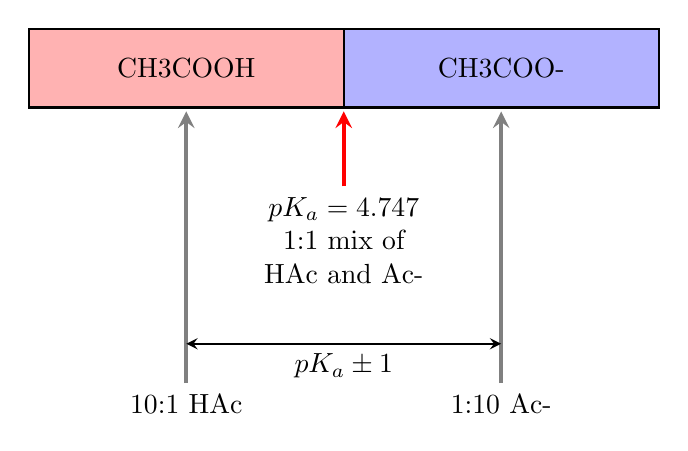
\begin{tikzpicture}
		\draw[thick,fill=red!30] (0,0) rectangle (4,1) node[pos=0.5]
		{\ch{CH3COOH}};
		\draw[thick,fill=blue!30] (4,0) rectangle (8,1) node[pos=0.5]
		{\ch{CH3COO-}};
		\draw[->,>=stealth,ultra thick,red] (4,-1) -- (4,-0.05)
		node[pos=0,black,below,align=center] {$\text{p}K_a = 4.747$ \\
		1:1 mix of \\ \ch{HAc} and \ch{Ac-}};
		\draw[->,>=stealth,ultra thick,gray] (2,-3.5) -- (2,-0.05)
		node[pos=0,black,below,align=center] {10:1 \ch{HAc}};
		\draw[->,>=stealth,ultra thick,gray] (6,-3.5) -- (6,-0.05)
		node[pos=0,black,below,align=center] {1:10 \ch{Ac-}};
		\draw[<->,>=stealth,thick,black] (2,-3) -- (6,-3)
		node[midway,below] {$\text{p}K_a \pm 1$};
	\end{tikzpicture}
	\end{center}

	For a monoprotic species, the weak acid predominates when $\text{pH} <
	\text{p}K_a$ and the weak base predominates when $\text{pH} >
	\text{p}K_a$.
	}


	\only<+>{%
	What about polyprotic species?

	\begin{center}
	\begin{tikzpicture}
		\draw[thick,fill=red!50] (0,0) rectangle (2,1) node[pos=0.5]
		{\ch{H3A}};
		\draw[thick,fill=red!30] (2,0) rectangle (4,1) node[pos=0.5]
		{\ch{H2A-}};
		\draw[thick,fill=blue!30] (4,0) rectangle (6,1) node[pos=0.5]
		{\ch{HA^{2-}}};
		\draw[thick,fill=blue!50] (6,0) rectangle (8,1) node[pos=0.5]
		{\ch{A^{3-}}};
		\draw[->,>=stealth,ultra thick,gray] (2,-1) -- (2,-0.05)
		node[pos=0,black,below] {$\text{p}K_1$};
		\draw[->,>=stealth,ultra thick,gray] (4,-1) -- (4,-0.05)
		node[pos=0,black,below] {$\text{p}K_2$};
		\draw[->,>=stealth,ultra thick,gray] (6,-1) -- (6,-0.05)
		node[pos=0,black,below] {$\text{p}K_3$};
		\draw[->,>=stealth,ultra thick,gray] (3,-3) -- (3,-0.05)
		node[pos=0,black,left,align=right] {$\text{pH} =
		\frac{1}{2}(\text{p}K_1 + \text{p}K_2)$ \\ $[\ch{H3A}] =
		[\ch{HA^{2-}}]$};
		\draw[->,>=stealth,ultra thick,gray] (5,-3) -- (5,-0.05)
		node[pos=0,black,right,align=left] {$\text{pH} =
		\frac{1}{2}(\text{p}K_2 + \text{p}K_3)$ \\ $[\ch{H2A-}] =
		[\ch{A^{3-}}]$};
		\node at (4,1.5) {pH};
		\draw[->,>=stealth,ultra thick] (2,1.5) -- (1,1.5)
		node[pos=0,right,align=center] {More \\ acidic};
		\draw[->,>=stealth,ultra thick] (6,1.5) -- (7,1.5)
		node[pos=0,left,align=center] {More \\ basic};
	\end{tikzpicture}
	\end{center}
}
\end{frame}

\begin{frame}[t]{What about all of the other species?}
	We can use \alert{fractional composition} equations and diagrams!
%
%	\bigskip
%
%	For monoprotic systems: 
%	\begin{align*}
%		\ch{HA + H2O <=> H3O+ + A-} \qquad K_a =
%		\frac{[\ch{H3O+}][\ch{A-}]}{[\ch{HA}]}
%	\end{align*}
%	\begin{align*}
%		\shortintertext{Mass balance:}
%		\si{\formal} &= [\ch{HA}] + [\ch{A-}] \\
%		\shortintertext{Some substitution:}
%		K_a &= \frac{[\ch{H3O+}](\si{\formal} - [\ch{HA}])}{[\ch{HA}]}
%		\\
%		\shortintertext{And rearranging:}
%		[\ch{HA}] &= \frac{[\ch{H3O+}]\si{\formal}}{[\ch{H3O+}] + K_a}
%		\\
%		\shortintertext{\framebreak If we divide by \si{\formal}\ldots}
%		\underbrace{\frac{[\ch{HA}]}{\si{\formal}}}_{\mathclap{\alpha_{\ch{HA}}
%		= \frac{[\ch{HA}]}{\si{\formal}}}}% \\ \text{Fraction of
%		%Dissociation!}}}
%		&= \frac{[\ch{H3O+}]}{[\ch{H3O+}] + K_a} \\
%		\shortintertext{Thus,}
%		\alpha_{\ch{HA}} &= \frac{[\ch{H3O+}]}{[\ch{H3O+}] + K_a} \\
%		\shortintertext{and}
%		\alpha_{\ch{A-}} &= \frac{K_a}{[\ch{H3O+}] + K_a}
%	\end{align*}
\end{frame}

\begin{frame}{Fractional Composition of Acetic Acid}
	\begin{columns}
		\column{0.3\textwidth}
		\begin{align*}
			\alpha_{\ch{HA}} &= \frac{[\ch{H3O+}]}{[\ch{H3O+}] +
			K_a} \\
			\alpha_{\ch{A-}} &= \frac{K_a}{[\ch{H3O+}] + K_a}
		\end{align*}
		\column{0.6\textwidth}
		\begin{center}
		\documentclass{standalone}

\usepackage{tikz}
\usepackage{pgfplots}
\usepackage{mathtools}
\usepackage{mhchem}
\usepackage{siunitx}
\DeclareSIUnit{\Molar}{\textsc{m}}

\setlength{\textwidth}{3in}
\setlength{\textheight}{4in}

\begin{document}

\begin{tikzpicture}
	\begin{axis} [
			width=\linewidth,
			height=18em,
			xmax=9,
			xmin=1,
			ymax=1,
			ymin=0,
			xlabel={pH},
			ylabel={$\alpha$},
			label style={font=\footnotesize},
			tick label style={font=\footnotesize},
			xtick={1,2,...,9},
			ytick={0.0,0.1,...,4},
			no markers,
    			every axis plot/.append style={ultra thick},
			]
		\addplot table [
			x=pH,
			y=HA,
			col sep=comma
			]
		{aceticacidfrac.csv} node at (axis cs:2,0.9)
		{$\alpha_{\ch{HA}}$};
		\addplot table [
			x=pH,
			y=A,
			col sep=comma
			]
			{aceticacidfrac.csv} node at (axis cs:8,0.9)
			{$\alpha_{\ch{A-}}$} node[right,black] at (axis cs:4.74,0.5) {$\leftarrow \text{p}K_a$};
	\end{axis}
\end{tikzpicture}

\end{document}

		\end{center}
	\end{columns}
\end{frame}

\vspace{\stretch{-1}}
\clearpage

\begin{frame}[allowframebreaks]{Fractional Composition of Diprotic Systems}
	\begin{align*}
		\ch{H2A + H2O &<=> H3O+ + HA-} \qquad &K_{a1} &=
		\frac{[\ch{H3O+}][\ch{HA-}]}{[\ch{H2A}]} \\
		\ch{HA- + H2O &<=> H3O+ + A^{2-}} \qquad &K_{a2} &=
		\frac{[\ch{H3O+}][\ch{A^{2-}}]}{[\ch{HA-}]}
	\end{align*}
	\begin{align*}
		\shortintertext{Mass Balance:}
		\si{\formal} &= [\ch{H2A}] + [\ch{HA-}] + [\ch{A^{2-}}] \\
		\shortintertext{Rearranging $K_{a1}$:}
		[\ch{HA-}] &= \frac{[\ch{H2A}]K_{a1}}{[\ch{H3O+}]} \\
		\shortintertext{Rearranging $K_{a2}$:}
		[\ch{A^{2-}}] &= \frac{[\ch{HA-}]K_{a2}}{[\ch{H3O+}]} =
		\frac{[\ch{H2A}]K_{a1}K_{a2}}{[\ch{H3O+}]} \\
		\shortintertext{\framebreak So the mass balance becomes:}
		\si{\formal} &= [\ch{H2A}] +
		\frac{[\ch{H2A}]K_{a1}}{[\ch{H3O+}]} +
		\frac{[\ch{H2A}]K_{a1}K_{a2}}{[\ch{H3O+}]} \\
		\shortintertext{or}
		\si{\formal} &= [\ch{H2A}]\bigg(1 + \frac{K_{a1}}{[\ch{H3O+}]}
		+ \frac{K_{a1}K_{a2}}{[\ch{H3O+}]}\bigg) \\
		\shortintertext{Therefore,}
		\alpha_{\ch{H2A}} &= \frac{[\ch{H2A}]}{\si{\formal}} =
		\frac{[\ch{H3O+}]^2}{[\ch{H3O+}]^2 + [\ch{H3O+}]K_{a1} +
		K_{a1}K_{a2}} \\[0.5em]
		\alpha_{\ch{HA-}} &= \frac{[\ch{HA-}]}{\si{\formal}} =
		\frac{K_{a1}[\ch{H3O+}]}{[\ch{H3O+}]^2 + [\ch{H3O+}]K_{a1} +
		K_{a1}K_{a2}} \\[0.5em]
		\alpha_{\ch{A^{2-}}} &= \frac{[\ch{A^{2-}}]}{\si{\formal}} =
		\frac{K_{a1}K_{a2}}{[\ch{H3O+}]^2 + [\ch{H3O+}]K_{a1} +
		K_{a1}K_{a2}}
	\end{align*}
\end{frame}

\begin{frame}{Fractional Composition of Fumaric Acid}
	\begin{center}
		\documentclass{standalone}

\usepackage{tikz}
\usepackage{pgfplots}
\usepackage{mathtools}
\usepackage{mhchem}
\usepackage{siunitx}
\DeclareSIUnit{\Molar}{\textsc{m}}

\setlength{\textwidth}{3in}
\setlength{\textheight}{4in}

\begin{document}

\begin{tikzpicture}
	\begin{axis} [
			width=\linewidth,
			height=18em,
			xmax=7.25,
			xmin=0,
			ymax=1,
			ymin=0,
			xlabel={pH},
			ylabel={$\alpha$},
			label style={font=\footnotesize},
			tick label style={font=\footnotesize},
			xtick={0,1,...,8},
			ytick={0.0,0.1,...,4},
			no markers,
    			every axis plot/.append style={ultra thick},
			]
		\addplot table [
			x=pH,
			y=H2A,
			col sep=comma
			]
		{fumaricacidfrac.csv} node at (axis cs:1,0.9)
		{$\alpha_{\ch{H2A}}$};
		\addplot table [
			x=pH,
			y=HA,
			col sep=comma
			]
			{fumaricacidfrac.csv} node at (axis cs:3.95,0.8)
			{$\alpha_{\ch{HA}}$} node[black,left] at (axis
			cs:3.02,0.5) {$\text{p}K_{a1} = 3.02 \rightarrow$};
		\addplot table [
			x=pH,
			y=A,
			col sep=comma
			]
			{fumaricacidfrac.csv} node at (axis cs:6.5,0.9)
			{$\alpha_{\ch{A-}}$} node[right,black] at (axis
			cs:4.48,0.5) {$\leftarrow \text{p}K_{a2} = 4.48$};
	\end{axis}
\end{tikzpicture}

\end{document}

	\end{center}
\end{frame}

\begin{frame}{What about polyprotic species?}
	\begin{block}{General Form for \ch{H_{$n$}A}}
		\begin{align*}
		\alpha_{\ch{H_{$n-j$}A}} = \frac{K_1 K_2 \cdots K_j
		[\ch{H3O+}]^{n-j}}{
			\begin{multlined}
				[\ch{H3O+}]^n + K_1 [\ch{H3O+}]^{n-1} + K_1K_2
				[\ch{H3O+}]^{n-2} \\ + \cdots + K_1 K_2 K_3
				\cdots K_n
			\end{multlined}
			}
		\end{align*}

		\bigskip

		\begin{center}
			(or take a look at Table 11-5, pg. 264,
			10\textsuperscript{th} Ed.)
		\end{center}
	\end{block}
\end{frame}

\begin{frame}{Fractional Composition of Glutamic Acid}
	\begin{center}
		\documentclass{standalone}

\usepackage{tikz}
\usepackage{pgfplots}
\usepackage{mathtools}
\usepackage{mhchem}
\usepackage{siunitx}
\DeclareSIUnit{\Molar}{\textsc{m}}

\setlength{\textwidth}{3in}
\setlength{\textheight}{4in}

\begin{document}

\begin{tikzpicture}
	\begin{axis} [
			width=\linewidth,
			height=18em,
			xmax=13.5,
			xmin=0,
			ymax=1,
			ymin=0,
			xlabel={pH},
			ylabel={$\alpha$},
			label style={font=\footnotesize},
			tick label style={font=\footnotesize},
			xtick={0,1,...,14},
			ytick={0.0,0.1,...,4},
			no markers,
    			every axis plot/.append style={ultra thick},
			]
		\addplot table [
			x=pH,
			y=H3A,
			col sep=comma
			]
		{glutamicacidfrac.csv} node at (axis cs:0.5,0.9)
		{$\alpha_{\ch{H3A+}}$};
		\addplot table [
			x=pH,
			y=H2A,
			col sep=comma
			]
			{glutamicacidfrac.csv} node at (axis cs:3.5,0.9)
			{$\alpha_{\ch{H2A}}$} node[black,left] at (axis
			cs:2.16,0.5) {$\text{p}K_{a1} \rightarrow$};
		\addplot table [
			x=pH,
			y=HA,
			col sep=comma
			]
			{glutamicacidfrac.csv} node at (axis cs:7,0.9)
			{$\alpha_{\ch{HA}}$} node[black,right] at (axis
			cs:4.30,0.5) {$\leftarrow \text{p}K_{a2}$};
		\addplot table [
			x=pH,
			y=A,
			col sep=comma
			]
			{glutamicacidfrac.csv} node at (axis cs:12.25,0.9)
			{$\alpha_{\ch{A-}}$} node[right,black] at (axis
			cs:9.96,0.5) {$\leftarrow \text{p}K_{a3}$};
	\end{axis}
\end{tikzpicture}

\end{document}

	\end{center}
\end{frame}

\begin{frame}{Can we draw a diagram without all of the equations?}
	\pause

	\alert{Yes!}

	\begin{itemize}
		\item At every $\alpha_n = 0.50$, $\text{pH} = \text{p}K_a$.
		\item From Henderson-Hasselbalch, we know
			\begin{itemize}
				\item at $\text{pH} = \text{p}K_a \pm 1$, we
					have 10:1 excess of something.
				\item at $\text{pH} = \text{p}K_a \pm 2$, we
					have 100:1 excess of something.
				\item at $\text{pH} = \text{p}K_a \pm 3$, we
					assume that we must be nearing
					\alert{100\%} of a principal component.
			\end{itemize}
	\end{itemize}
\end{frame}

\begin{frame}{An Example: Drawing $\alpha_{\text{Histidine}}$}
	\begin{center}
		\only<1>{\includegraphics[width=0.6\textwidth]{histidine.png}}
		
		\only<2>{\documentclass{standalone}

\usepackage{tikz}
\usepackage{pgfplots}
\usepackage{mathtools}
\usepackage{mhchem}
\usepackage{siunitx}
\DeclareSIUnit{\Molar}{\textsc{m}}

\setlength{\textwidth}{3in}
\setlength{\textheight}{4in}

\begin{document}

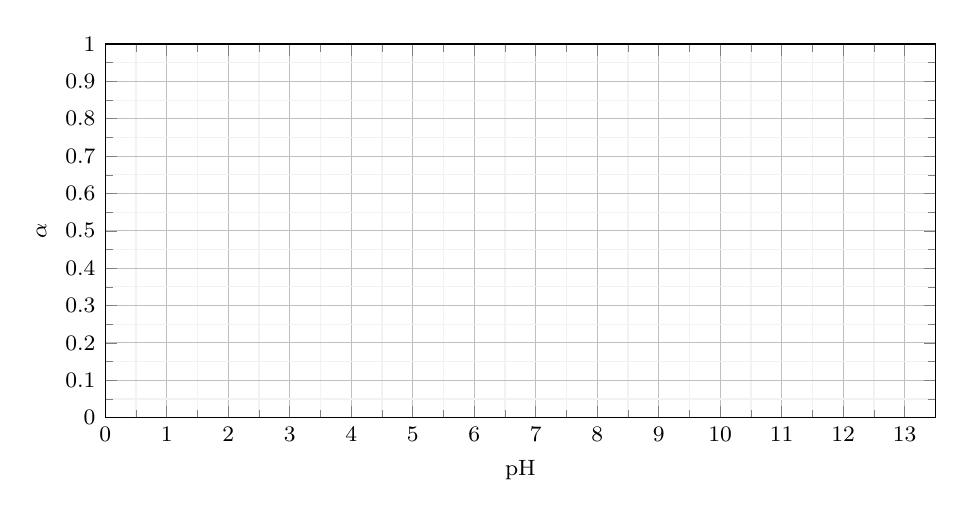
\begin{tikzpicture}
	\begin{axis} [
			width=\linewidth,
			height=18em,
			grid=both,
			minor tick num=1,
			major grid style={draw=gray!50},
			minor grid style={draw=gray!10},
			xmax=13.5,
			xmin=0,
			ymax=1,
			ymin=0,
			xlabel={pH},
			ylabel={$\alpha$},
			label style={font=\footnotesize},
			tick label style={font=\footnotesize},
			xtick={0,1,...,14},
			ytick={0.0,0.1,...,4},
			no markers,
    			every axis plot/.append style={ultra thick},
			]
	\end{axis}
\end{tikzpicture}

\end{document}
}
		\note<2>{\documentclass{standalone}

\usepackage{tikz}
\usepackage{pgfplots}
\usepackage{mathtools}
\usepackage{mhchem}
\usepackage{siunitx}
\DeclareSIUnit{\Molar}{\textsc{m}}

\setlength{\textwidth}{3in}
\setlength{\textheight}{4in}

\begin{document}

\begin{tikzpicture}
	\begin{axis} [
			width=\linewidth,
			height=18em,
			grid=both,
			minor tick num=1,
			major grid style={draw=gray!50},
			minor grid style={draw=gray!10},
			xmax=13.5,
			xmin=0,
			ymax=1,
			ymin=0,
			xlabel={pH},
			ylabel={$\alpha$},
			label style={font=\footnotesize},
			tick label style={font=\footnotesize},
			xtick={0,1,...,14},
			ytick={0.0,0.1,...,4},
			no markers,
    			every axis plot/.append style={ultra thick},
			]
			\visible<+(2)->{
		\addplot table [
			x=pH,
			y=H3A,
			col sep=comma
			]
		{histidinefrac.csv};
		\addplot table [
			x=pH,
			y=H2A,
			col sep=comma
			]
			{histidinefrac.csv};
		\addplot table [
			x=pH,
			y=HA,
			col sep=comma
			]
			{histidinefrac.csv};
		\addplot table [
			x=pH,
			y=A,
			col sep=comma
			]
			{histidinefrac.csv};
		}
	\end{axis}
\end{tikzpicture}

\end{document}
}
%		\only<2->{\documentclass{standalone}

\usepackage{tikz}
\usepackage{pgfplots}
\usepackage{mathtools}
\usepackage{mhchem}
\usepackage{siunitx}
\DeclareSIUnit{\Molar}{\textsc{m}}

\setlength{\textwidth}{3in}
\setlength{\textheight}{4in}

\begin{document}

\begin{tikzpicture}
	\begin{axis} [
			width=\linewidth,
			height=18em,
			grid=both,
			minor tick num=1,
			major grid style={draw=gray!50},
			minor grid style={draw=gray!10},
			xmax=13.5,
			xmin=0,
			ymax=1,
			ymin=0,
			xlabel={pH},
			ylabel={$\alpha$},
			label style={font=\footnotesize},
			tick label style={font=\footnotesize},
			xtick={0,1,...,14},
			ytick={0.0,0.1,...,4},
			no markers,
    			every axis plot/.append style={ultra thick},
			]
			\visible<+(2)->{
		\addplot table [
			x=pH,
			y=H3A,
			col sep=comma
			]
		{histidinefrac.csv};
		\addplot table [
			x=pH,
			y=H2A,
			col sep=comma
			]
			{histidinefrac.csv};
		\addplot table [
			x=pH,
			y=HA,
			col sep=comma
			]
			{histidinefrac.csv};
		\addplot table [
			x=pH,
			y=A,
			col sep=comma
			]
			{histidinefrac.csv};
		}
	\end{axis}
\end{tikzpicture}

\end{document}
}
	\end{center}

%	\note<2>{
%		\documentclass{standalone}

\usepackage{tikz}
\usepackage{pgfplots}
\usepackage{mathtools}
\usepackage{mhchem}
\usepackage{siunitx}
\DeclareSIUnit{\Molar}{\textsc{m}}

\setlength{\textwidth}{3in}
\setlength{\textheight}{4in}

\begin{document}

\begin{tikzpicture}
	\begin{axis} [
			width=\linewidth,
			height=18em,
			grid=both,
			minor tick num=1,
			major grid style={draw=gray!50},
			minor grid style={draw=gray!10},
			xmax=13.5,
			xmin=0,
			ymax=1,
			ymin=0,
			xlabel={pH},
			ylabel={$\alpha$},
			label style={font=\footnotesize},
			tick label style={font=\footnotesize},
			xtick={0,1,...,14},
			ytick={0.0,0.1,...,4},
			no markers,
    			every axis plot/.append style={ultra thick},
			]
			\visible<+(2)->{
		\addplot table [
			x=pH,
			y=H3A,
			col sep=comma
			]
		{histidinefrac.csv};
		\addplot table [
			x=pH,
			y=H2A,
			col sep=comma
			]
			{histidinefrac.csv};
		\addplot table [
			x=pH,
			y=HA,
			col sep=comma
			]
			{histidinefrac.csv};
		\addplot table [
			x=pH,
			y=A,
			col sep=comma
			]
			{histidinefrac.csv};
		}
	\end{axis}
\end{tikzpicture}

\end{document}

%	}
\end{frame}

\begin{frame}{What purpose does this serve besides titrations?}
	Proteins can be separated by charge.
	\begin{center}
		\includegraphics[width=0.6\textwidth]{alanine.png}
	\end{center}

	\begin{itemize}
			\only<1>{
		\item Isoionic Point
			\begin{itemize}
				\item the pH of the pure, neutral, polyprotic
					acid (the neutral zwitterion).
					\only<1|handout:0>{
					\begin{itemize}
						\item[Example:] Alanine
							dissolved in pure water
							is neutral and
							equilibrium creates
							\alert{non-equal}
							concentrations of
							\ch{H2A+} and \ch{A-}.
					\end{itemize}
					}
			\end{itemize}}
			\only<2>{
		\item Isoelectric Point
			\begin{itemize} 
				\item the pH at which average charge of the
					polyprotic acid is 0.
					\only<2|handout:0>{
					\begin{itemize}
						\item[Example:] Alanine is
							dissolved in pure water,
							but NaOH/HCl is added to
							adjust the pH so that
							\alert{[\ch{H2A+}] =
							[\ch{A-}]}.
					\end{itemize}
					}
			\end{itemize}}
	\end{itemize}
\end{frame}

\begin{frame}{Isoionic and Isoelectric Points of Alanine}
\note{
	\begin{itemize}
		\item \textbf{Isoionic Point:}
			\begin{align*}
				[\ch{H3O+}] &= \sqrt{\frac{K_1K_2\si{\formal} +
				K_1K_w}{K_1 + \si{\formal}}} \\
				\intertext{For \SI{0.10}{\Molar} alanine,}
				[\ch{H3O+}] &= \SI{7.7e-7}{\Molar} \therefore
				\text{pH} = \fbox{6.11}
			\end{align*}
\end{itemize}}
\end{frame}

\note{\begin{itemize}
		\item \textbf{Isoelectric Point:}
			\begin{align*}
				\shortintertext{We need}
				[\ch{H2A+}] &= [\ch{A-}] \\
				\shortintertext{Rearranging $K$,}
				[\ch{H2A+}] &=
				\frac{[\ch{H3O+}][\ch{HA}]}{K_1} \\
				[\ch{A-}] &= \frac{K_2[\ch{HA}]}{[\ch{H3O+}]}
				\\
				\shortintertext{Setting the two equal to each
				other,} \frac{[\ch{H3O+}][\ch{HA}]}{K_1} =
				\frac{K_2[\ch{HA}]}{[\ch{H3O+}]} &\rightarrow
				[\ch{H3O+}] = \sqrt{K_1K_2} \\
				\shortintertext{\textit{This looks
				familiar\ldots}}
				\text{pH} &= \frac{1}{2}(\text{p}K_1 +
				\text{p}K_2) = \fbox{6.10}
			\end{align*}
	\end{itemize}}

	\mode<article>{\vfill}

\begin{frame}{Isoelectric Focusing of Proteins}
	\only<+>{%
	\begin{columns}
		\column{0.45\textwidth}
		\begin{enumerate}
			\item A gel is submerged in a conducting solution and
				several hundred volts are applied.
			\item The potential difference introduces a pH gradient
				across the gel.
			\item The proteins distribute themselves according to
				isoelectric point because.
				%, as neutral species,
				%they are no longer attracted to either
				%electrode.
		\end{enumerate}
		\column{0.45\textwidth}
		\begin{center}
		\includegraphics[scale=0.85]{whitford-isoelectric.png}
	\end{center}

		\bigskip

		{\footnotesize Whitford, D. \textit{Proteins: Structure and
		Function}; Wiley: Hoboken, NJ, 2005.}

	\end{columns}
	}

	\only<+>{%
	\mode<presentation>{
	\begin{center}
		\includegraphics[width=\linewidth]{harris-isoelectric.png}
	\end{center}
	{\footnotesize Harris, 9\textsuperscript{th} Ed.}

	\bigskip

	\begin{itemize}
		\item A similar effect can be acheived in microfluidic channels
			using \alert{much smaller} sample volumes.
\end{itemize}}
}
\end{frame}

\end{document}
